\documentclass[a4paper,11pt]{scrartcl}
\usepackage[ngerman]{babel}
\usepackage[utf8]{inputenc}

\usepackage{amssymb}
\usepackage{amsmath}
\usepackage{commath}

\usepackage[ngerman]{cleveref}
\usepackage{graphicx}
\usepackage{enumitem}

\newcommand*{\eps}{\varepsilon}
\newcommand*{\sm}{\sum_{i=0}^\infty}
\newcommand*{\Ld}{\mathcal{O}}
\newcommand*{\pyi}[1]{\frac{\partial{#1}}{\partial y_i}}
\newcommand*{\pxj}[1]{\frac{\partial{#1}}{\partial x_j}}
\newcommand*{\Dx}{\Delta{}x}

\setlist[enumerate,2]{label=\textbf{\alph*)}}


\begin{document}
\begin{enumerate}[label*=\textbf{9.\arabic*.}]

% ==================== 9.1 ====================
\item
  \begin{enumerate}
  \item
    DGL als System:
    \[\begin{pmatrix}y'\\v'\end{pmatrix}=
      \begin{pmatrix}v\\-\eps v^3 - y\end{pmatrix}
    \]
    Linearisiert ist der 0 punkt ein Zentrum.
    Der nichtlineare Anteil hilft zusäzlich die Lösung beschränkt zu halten.
    Sieht man in der Skizze vom Phasenportrait in \cref{fig:phaseportrait_9.1a}.

    \begin{figure}
    \centering
    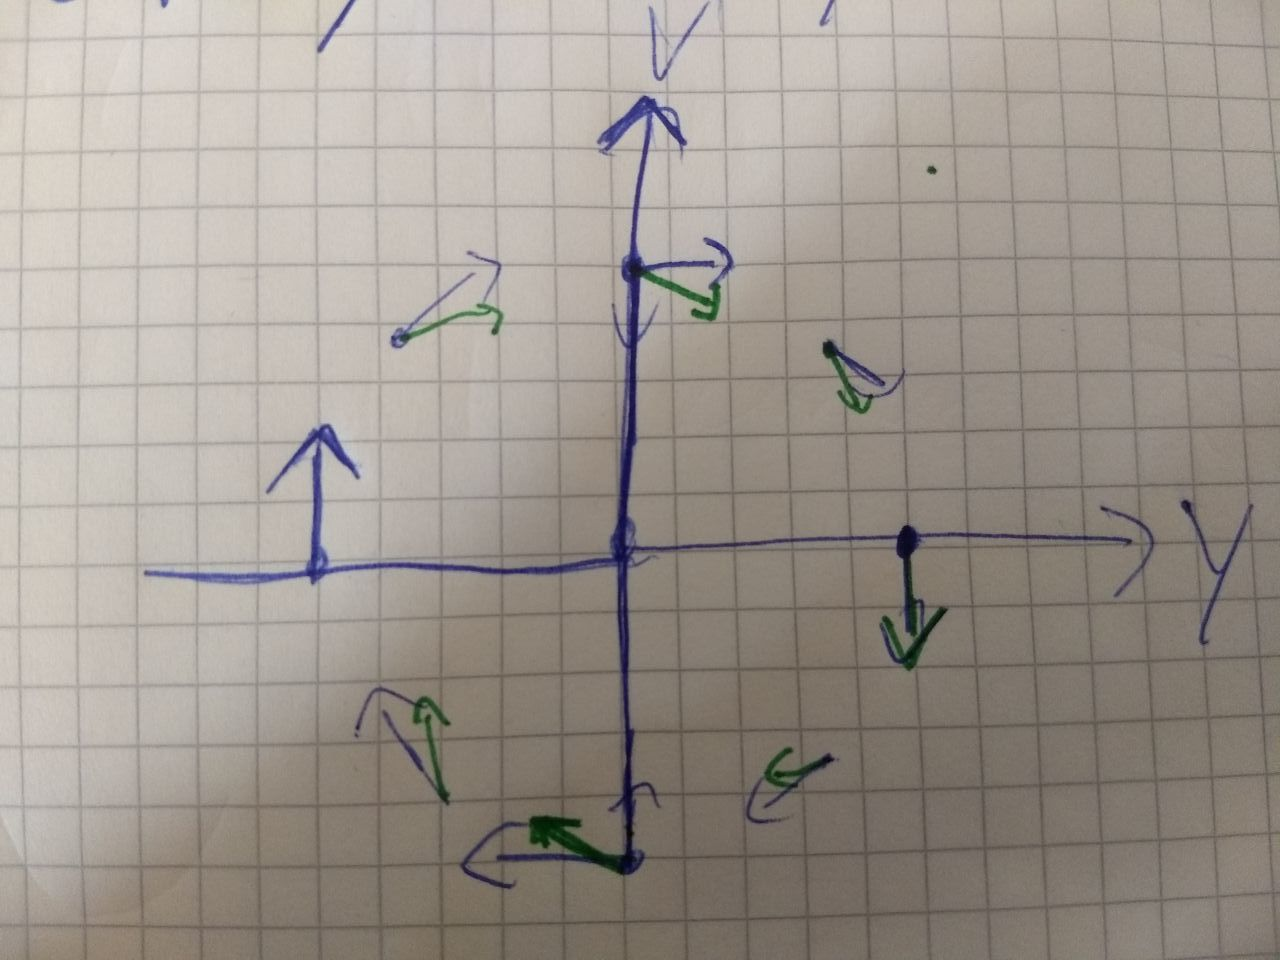
\includegraphics[width=.5\linewidth]{1a.jpg}
    \captionof{figure}{Skizze des Phasenportraits von 9.1a), blau: linearisiert, grün: nichtlinear}
    \label{fig:phaseportrait_9.1a}
    \end{figure}

  \item
    Mehrskalenansatz:
    \[ y = \sm \eps^i y_i(t, T), \quad \text{mit } T = \eps t \]
    \[ \Rightarrow y' = \sm \eps^i \partial_{1} y_i + \eps^{i+1} \partial_2 y_i\]
    \[ \Rightarrow y'' = \sm \eps^i \partial_{11} y_i + \eps^{i+1} \partial_{12}
      y_i + \eps^{i+1} \partial_{21} y_i + \eps^{i+2} \partial_{22} y_i\]

    Die DGL für den $\eps^0$ Term ist:
    \[ \partial_{11} y_0 + y_0 = 0\]
    Wie in der Vorlesung schreiben wir die allgemeine Lösung dafür als:
    \[ y_0 = r(T) \cos(t + \varphi(T))\]
    Die DGL für den $\eps^1$ Term ist:
    \[\partial_{11} y_1 + y_1 = - (\partial_1 y_0)^3 -2 \partial_{12} y_0\]
    \[\partial_1 y_0 = r(T) \sin(t+\varphi(T)), \quad (\partial_1 y_0)^3 =
      r^3(T) \frac{3 \sin(t + \varphi(T)) - \sin(3 (t + \varphi(T))}{4}\]
    \[\partial_{12} y_0 = r'(T) \sin(t+\varphi(T)) - r(T) \cos(t + \varphi(T)) \varphi'(T) \]

    Daher ist die rechte Seite der $\eps^1$-Gleichung:
    \[\left(2r'(T) + \frac{3}{4} r^3(T)\right) \sin(t + \varphi(T)) - r(T) \varphi'(T) \cos(t
     + \varphi(T)) - 2r^3(T) \sin(3(t + \varphi(T))) \]

   Damit $y_1$ kein Wachstum in $t$ hat setzen wir die Terme vor den Lösungen der
   homogenen Gleichung auf 0.
   ($\sin(t), \cos(t)$ würden die homogene Gleichung lösen; $\sin(3t)$ nicht).
   \[ 2r'(T) + \frac{3}{4}r^3(T) = 0, \quad -r(T)\varphi'(T) = 0\]
   Die erste Gleichung kann mittels Variablenseparation gelöst werden und die
   \[ r = \frac{1}{\sqrt{\frac{6}{8}T + c_1}}\]
   Aus der zweiten Gleichungt folgt $\varphi'(T) = 0 \Rightarrow \varphi(T) \equiv c_2$.

   Also
   \[y_0(t) = \frac{1}{\sqrt{\frac{6}{8}\eps t + c_1}} \cos(t + c_2)\]

   Die Konstanten können aus den Anfangsbedingungen ermittelt werden:
   \[a = y_0(0) = \frac{1}{\sqrt{c_1}} \cos(c_2) \Rightarrow
     (c_1)^{-\frac{1}{2}} = \frac{a}{\cos(c_2)}\]
   \[y'_0(t) = -\frac{3}{8}\eps \left(\frac{6}{8}\eps t +
       c_1\right)^{-\frac{3}{2}} \cos(t+c_2)- \left(\frac{6}{8}\eps t +
       c_1\right)^{-\frac{1}{2}} \sin(t + c_2)\]
   \[0 = y'_0(0) = -\frac{3}{8}\eps \left(c_1\right)^{-\frac{3}{2}} \cos(c_2)
     - \left(c_1\right)^{-\frac{1}{2}} \sin(c_2)
   = -\frac{3}{8} \eps \frac{a^3}{\cos^3(c_2)} \cos(c_2) - \frac{a\sin(c_2)}{\cos(c_2)}\]
 \[-\frac{3}{8} \eps a^2 = \sin(c_2)\cos(c_2) = \frac{1}{2}\sin(2c_2)\]
 \[c_2 = \frac{1}{2}\arcsin\left(\frac{-3}{8}\eps a^2\right)\]

\end{enumerate}


% ==================== 9.2 ====================
\item \begin{enumerate}
  \item
  \item
\end{enumerate}


% ==================== 9.3 ====================
\item


% ==================== 9.4 ====================
\item


% ==================== 9.5 ====================
\item \begin{enumerate}
  \item
    In jedem Punkt ist $\nabla \varphi(x)$ eine orthogonale Matrix $Q(x)$,
    da $\nabla\varphi(x)^{-1} = (\nabla \varphi(x))^\top$.
    Außerdem gilt auch $C_{\varphi^{-1}} \equiv I$, da $\nabla \varphi^{-1} =
    (\nabla \varphi)^{-1}$.

    Aus dem Angleitner Skript S. 29:
    \[
      \frac{\norm{\varphi(x+\Dx) - \varphi(x)}^2}{\norm{(x + \Dx) - x}^2}
    = \frac{\norm{\nabla\varphi(x)\cdot \Dx + \Ld(\norm{\Delta
          x}^2)}^2}{\norm{\Dx}^2}\]
    \[= \frac{(\Dx)^\top \cdot
      (\nabla\varphi(x))^\top \cdot (\nabla\varphi(x))\cdot \Dx}{\norm{\Delta
        x}^2} + \Ld(\norm{\Dx}) \overset{C=I}{=} 1 + \Ld(\norm{\Dx}) \]

  Wählt man nun $x + \Dx = y$ erhält man:
\[ \frac{\norm{\varphi(y) - \varphi(x)}^2}{\norm{y - x}^2} = 1 +
  \Ld(\norm{\Dx}) \]
Und das ganze für $\varphi^{-1}$:
\[ \frac{\norm{y - x}^2}{\norm{\varphi(y) - \varphi(x)}^2} = 1 +
  \Ld(\norm{\varphi(y)-\varphi(x)}) = 1 + \Ld(\norm{\Dx})\]

Also
\[ \frac{\norm{\varphi(y) - \varphi(x)}^2}{\norm{y - x}^2} = 1 +
  \Ld(\norm{\Dx}) = 1 + \Ld(\norm{\Dx}^{-1}) \]

Kann man daraus schließen, dass die $\norm{\Dx}$ Terme wegfallen?

Offene Frage: Wo geht Konvexität von $B$ ein?

  \item
    Aus \textbf{a)} gilt $G(x, y) = 0$.

    Zuerst nach $y_i$ und dann nach $x_j$ differenzieren führt zur gesuchten Identität:
    \[G(x, y) = \sum_k (\varphi_k(x) - \varphi_k(y))^2 - (x_k - y_k)^2 = 0\]
    \[\pyi{}G(x,y) = -2 \sum_k (\varphi_k(x) - \varphi_k(y)) \pyi{\varphi_k(y)}
      + 2 (x_i - y_i) = 0\]
    \[\pxj{}\pyi{}G(x,y) = -2 \sum_k \pyi{\varphi_k(y)} \pxj{\varphi_k(x)}
      + 2 \delta_{ij} = 0\]

    Also $(\nabla\varphi(y))^\top \nabla\varphi(x) = I$ auch für verschiedene
    Punkte $y, x \in B$.

  \item
    Es folgt, dass in konvexen Umgebungen von $x \in \Omega$ gilt: $(\nabla
    \varphi(y))^\top = \nabla \varphi(x)^{-1}$ und damit $\nabla \varphi(x) =
    \nabla \varphi(y)$. $\nabla\varphi$ ist lokal eine konstante orthogonale
    Matrix $Q$. Damit $\varphi(x) = Q x + a$.
\end{enumerate}

\end{enumerate}
\end{document}